\cleartooddpage[\thispagestyle{empty}]
\chapter{The Dark Matter Paradigm}

  As dark matter makes up 26.5\% of the universe's energy and 81.5\% of its mass \cite{planck2015}, it has had a significant impact on the development of the universe, shaping its present day distribution.

  {\color{red}(Should I show the following calculation into this paragraph to justify the above percentages??)}
  \begin{verbatim}
  From: https://arxiv.org/abs/1502.01589 , Table 3, column [4] :
    omega_b h^2 = 0.02225
    omega_c h^2 = 0.1198
    H_0         = 67.27 km / s / Mpc
    h           = H_0 / ( 100 km / s / Mpc ) = 0.6727
  thus:
    omega_b = 0.02225 / h^2 = 0.0491 =  4.9% of universe's energy is in baryonic matter
    omega_c = 0.1198  / h^2 = 0.2647 = 26.5% of universe's energy is in dark matter
    ( 26.5 - 4.9 ) / 26.5 = 81.5% of universe's mass is stored in dark matter
  \end{verbatim}

  In this chapter, the main features of dark matter physics are discussed.
  This includes the astrophysical evidence for the existance of dark matter, an outline of the current cosmological paradigm of $\Lambda$CDM and the Standard Model, as well as arguments for why dark matter may be in the form of a new, unknown particle.

\section{Astrophysical Evidence for Dark Matter}
  The current effects attributed to dark matter can be grouped into four different length scales.
  These effects also fall into one of three categories: gravity pulling on electromagnetic emitters, gravity bending background light, or by measuring the universe's total energy budget.
  On the smallest scales, concentrations of several thousand stars can be seen revolving around their center of mass, at a larger distribution of speeds than one would expect from the existing visible amount of matter.
  At larger scales the optical light from galaxies, as well as hydrogen lines, can be used to measure the amount of mass and its rotational velocity around the center of galaxies.
  At even larger scales, galaxy velocities can be measured and compared, x-ray telescopes can monitor the amount of hot gas, and mass-heavy areas of space will gravitationally lens background galaxies.
  At the the largest scale, the measurement of oscillations in the cosmic microwave background can be used to determine the amount of dark and baryonic matter.
  
  {\color{red}(supernovae??)}

  {\color{red}(quasar time delay images??)}
  % Quasar Microlensing at High Magnification and the Role of Dark Matter: Enhanced Fluctuations and Suppressed Saddle Points
  % schechter 2002

  {\color{red}(weak lensing??)}
  
  \subsection{$10^{19}\:\text{m}$ : Dwarf Galaxy Scale}\label{dm_dwarfscale}
    % 10^19m comes from: 
    % fornax dwarf spheroidal galaxy wiki page
    %    17' x 12.6' in solid angle, call it 15'
    %    140kpc away  
    %    140kpc * Tan(15') = 0.6kpc = 1.8*10^19m ~ 10^19m
    At scales of $\nicetilde 10^{19}$m, groups of thousands stars, called satellite galaxies or dwarf galaxies, lie at the edge of full size galaxies.
    An example dwarf galaxy is in Figure \ref{fig:sculptor}, the Sculptor Dwarf Galaxy, imaged in the optical frequencies by the MPG/ESO Telescope.
    Measuring the mass of these dwarf galaxies is done in two ways.
    In the first, telescopes observed the individual spectra of these stars, allowing for their line-of-sight velocity to be calculated \cite{dwarf_gal_red_giant}.
    By looking at the distribution of these velocities (the width of this distribution is called the velocity dispersion), the total mass of the dwarf galaxy can be inferred~\cite{dwarf_gal_vel_dispersion, dwarf_gal_vel_dispersion2}.
    What makes this possible is that the velocity dispersion of a group of stars is proportional to the total mass of the graviational well.
    This can be seen by applying the virial theorem and maxwell-boltzmann statistics.
    {\color{red}(You should actually explain what the virial theorem is and how maxwell-boltzmann statistics is applied... -Orel ??)}
    As this measurement relies on doppler-shifted spectral lines, and not their absolute brightness, this mass estimate is fairly resistant to changes in absolute brightness, either due to atmospheric variations during telescope observations, or to the amount of light-absorbing dust in the line-of-sight.

    \begin{figure}[ht]
      \includegraphics[width=0.9\textwidth]{images/sculptor/sculptor.eps}
      \caption[Sculptor Dwarf Galaxy]{
        The Sculptor Dwarf Galaxy \cite{sculptor_image}, imaged with the MPG/ESO telescope \cite{sculptor_paper}.
        This dwarf galaxy has a $\frac{M_\odot}{L_\odot}$ ratio of 15.3 \cite{sculptor_ml}.
      }
      \label{fig:sculptor}
    \end{figure}
    
    The second way to measure galaxy masses is by measuring the total brightness of a galaxy, and divide by the luminosity of the Sun $L_\odot$, around .
    This then indicates the number of solar masses $M_\odot$ contained in the galaxy, a measure of its baryonic (i.e. 'bright', not dark) mass.
    By comparing the total mass in the first way to the 'bright' mass in the second way, the mass-to-light ratio can be calculated, indicating the amount of dark matter present in the galaxy~\cite{faber_ml}.
    For these calculations, $M_\odot$ is taken as {\color{red}(??)} and $L_\odot$ is taken as {\color{red}(??)}.
    
    Dwarf galaxies have mass-to-light ratios of around 5-100 $\frac{M_\odot}{L_\odot}$, but can be as high as \nicetilde 1000~\cite{Simon2007_dwarfgalaxykeck}.
    A random assortment of Local Group dwarf galaxies and their $\frac{M_\odot}{L_\odot}$ is shown in Table \ref{tab:mlratios:dwarfgals}.
    {\color{red}(You should explain what L is (also M if it was not explained in the introduction).  Also, please expand the explanation. Say explicitly that the mass is measured in two different ways, one directly from the luminous material, the other from the rotation, etc. -Orel ??)}
    
    \begin{table}[]
      \centering
      \caption{$\frac{M_\odot}{L_\odot}$ ratios of various dwarf galaxy objects, taken from Ref. \cite{localdwarfs}.}
      \label{tab:mlratios:dwarfgals}
      \begin{tabular}{l r}
        Object      &  Mass, units of $\frac{M_\odot}{L_\odot}$ \\
        \hline
        IC 10       &  0.1 \\
        NGC 147     &  7.1 \\
        NGC 185     &  2.5 \\
        NGC 205     & 12   \\
        LGS 3       & 21   \\
        IC 1613     &  1.4 \\
        Carina      & 30   \\
        Antlia      &  7.4 \\
        Leo I       &  3.1 \\
        Sextans     & 34   \\
        Ursa Minor  & 60   \\
        Draco       & 58   \\
        Sagittarius & 22   \\
      \end{tabular}
    \end{table}
    
    As an additional piece of evidence for Dark Matter, dwarf galaxies near the Perseus cluster were studied.
    It was found that, with their baryonic mass alone, these dwarf galaxies would be ripped apart by the tidal disruption of the Perseus cluster.
    Observations of these dwarf galaxies indicate they remain intact, leading to the conclusion that the presence of Dark Matter is providing extra gravitational force~\cite{Penny2009}.
    
    \FloatBarrier

  \subsection{$10^{20}\:\text{m}$ : Galaxy Scale}
    %
    % galaxy rotation curve wiki page, M33 has curve measurements out to 50,000ly
    %   50,000ly = 4.7*10^20m ~ 10^20m
    At scales of $\nicetilde 10^{20}$m, the effects of Dark Matter on galaxies are observable.
    Within galaxies, the amount of light observed in a sector predicts a lower amount of mass, while observing the line-of-sight velocity predicts a higher amount of mass.
    
    In the first prediction technique, the total amount of light produced by a quadrant of a galaxy is measured with optical telescopes.
    Then, like in Subsection \ref{dm_dwarfscale}, the amount of light produced can be compared with the Sun as a standard mass-to-light ratio, allowing for a prediction of the amount of mass contained in that sector.
    Known mass-to-light ratios can then be used to calculate the total amount of mass within that quadrant.
    For example, in a survey of 25 galaxies in Ref. \cite{galaxy_mass_light_ratio}, most possesed a mass-to-light ratio of 1 to 10.

    In the second prediction technique, a galaxy's emission spectrum is observed at many positions around its disk (center, outer edges, etc).
    By comparing the orientation of the disk with the doppler-shifted position of well-known spectral lines, one can calculate the average velocity that each section is travelling at around the center of its galaxy, forming a rotation curve~\cite{rotation_curve_review,spiral_galaxy_rot_curve,milkyway_dm_evidence}.
    Newton's law of gravity can then be used to calculate the mass contained within a sphere of that same radius.
    This calculation ends up with a larger amount of mass than the one found simply from the total amount of light observed.
    
    In Figure \ref{fig:m33rotcurve}, a rotation curve from M33 observations is shown.
    It can be seen that the observed velocity curve (the datapoints) keeps increasing at larger radii.
    If the galaxy was only made of stars, then the rotation curve would follow the short dashed line.
    If the galaxy was only made of gas, then the rotation curve would instead follow the long dashed line.
    As these two major components do not combine to form the observed rotation curve, the presence of Dark Matter can account for the difference, shown as the dashed-dotted line~\cite{m33rotcurve}.
    
    \begin{figure}[ht]
      \includegraphics[width=0.9\textwidth]{images/m33rotcurve/m33rotcurve.eps}
      \caption[M33 Rotation Curve]{
        The rotation curve from M33, taken from \cite{m33rotcurve}.
        The solid line is the best fitting model to the observed velocity measurments.
        The short dashed line is the stellar disk contribution, the gas contribution is the long dashed line, and the dashed-dotted line is the dark matter contribution.
      }
      \label{fig:m33rotcurve}
    \end{figure}
    
    \begin{table}[]
      \centering
      \caption{$\frac{M_\odot}{L_\odot}$ ratios of various galactic-scale objects, taken from \cite{faber_ml}.}
      \label{tab:mlratios}
      \begin{tabular}{l r}
        Object          & Mass, units of $\frac{M_\odot}{L_\odot}$ \\
        \hline
        M31 (Andromeda) &  7.6  \\
        M33             &  4.5  \\
        M51             &  3.3  \\
        M81             &  8.5  \\
        NGC 801         &  2.4  \\
        NGC 2403        &  5.5  \\
        NGC 2841        & 10.6  \\
        NGC 4324        &  5.5  \\
        NGC 6822        &  0.58 \\
      \end{tabular}
    \end{table}
      
    From Ref. \cite{faber_ml}, a random sample of galaxies are shown alongside their mass-to-light ratios in Table \ref{tab:mlratios}.
    Our own Milky Way galaxy is measured to have a mass to light ratio of 10 $\frac{M_{\odot}}{L_{\odot}}$ {\color{red}(and?? cite??)}.
    Galaxy rotation curves can also be measured through weak gravitational lensing \cite{weak_lensing_2001} {\color{red}(expand??)}.

  \subsection{$10^{23}\:\text{m}$ : Galaxy Cluster Scale}
    %
    % galaxy cluster wiki page
    % 2-10 Mpc, call it 6Mpc = 1.85*10^23m ~ 10^23m
    At scales of $\nicetilde 10^{23}$m, Dark Matter's effects on galactic clusters becomes observable by comparing three techniques.
    In the first technique, galaxy clusters are massive enough to bend the images of background galaxies.
    The type and amount of bending can be used to determine the mass of the intermediate galaxy.

    X-Ray observations of galaxy clusters can measure the amount of hot baryonic mass.
    This has been shown distinctly in the Bullet Cluster\cite{bullet_cluster}.
    In this cluster, the total (baryonic+dark) mass was traced using gravitational lensing of background light.
    The baryonic mass was then traced with x-rays, which are emitted by ionized gas in the region.
    Figure \ref{fig:bullet} then shows these two masses overlayed.
    {\color{red}(This has to be expanded a little and clarified. Also, you should mention how this evidence is really important for theories suggesting different gravitational laws. -Orel ??)}

    \begin{figure}[ht]
      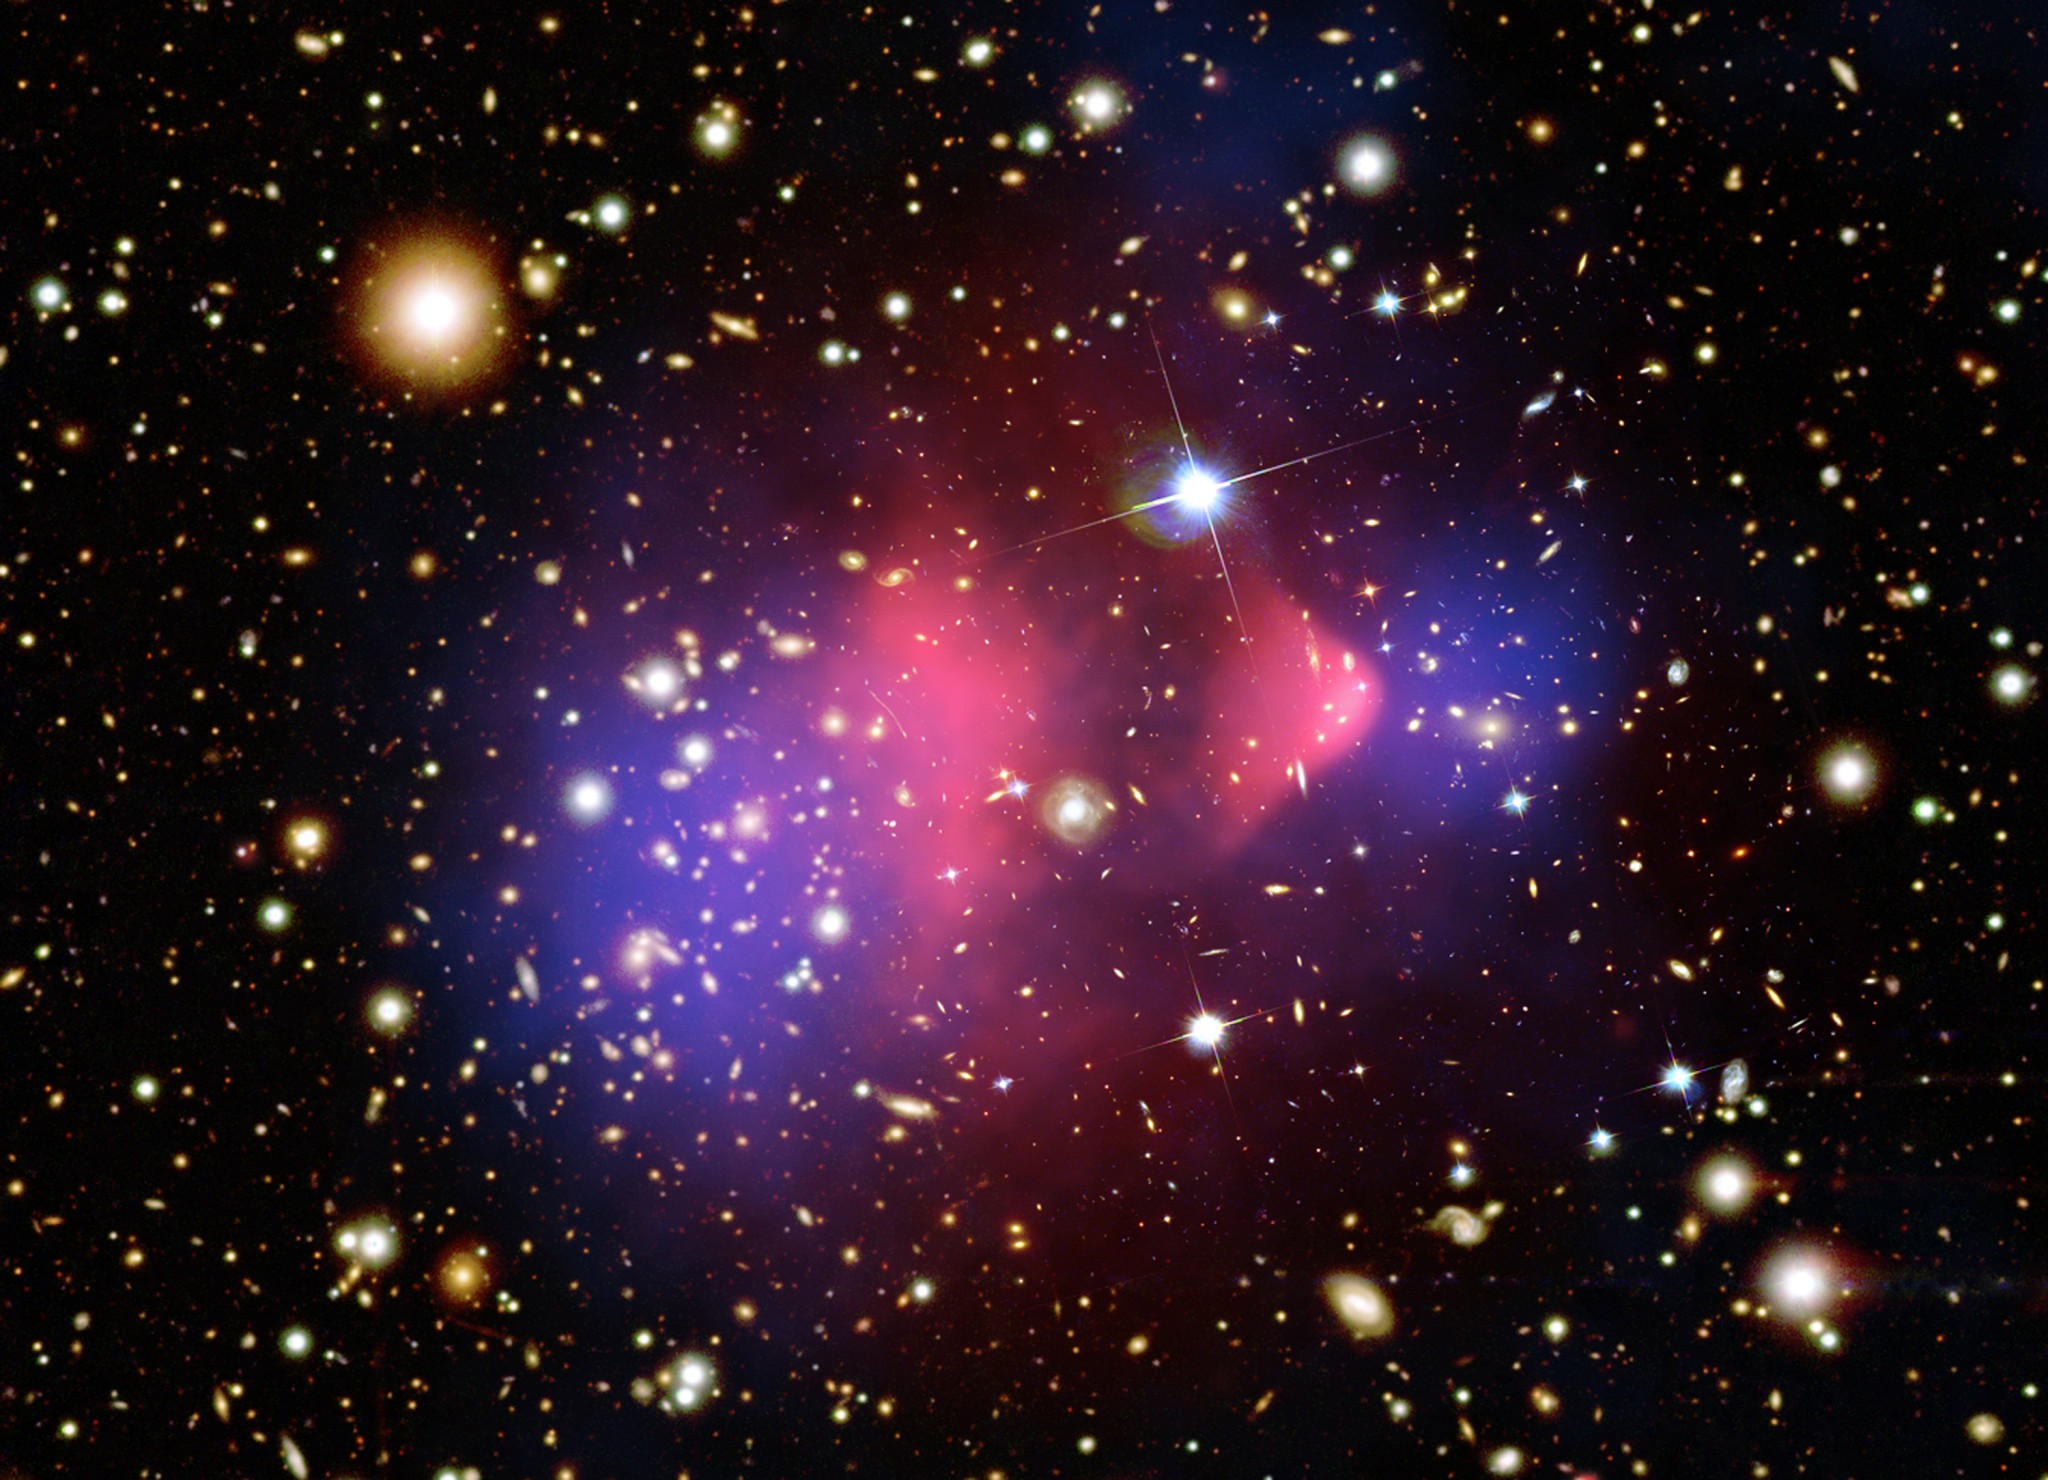
\includegraphics[width=0.95\textwidth]{images/bulletcluster.eps}
      \caption[The Bullet Cluster]{
        The bullet cluster\cite{bullet_cluster_combined_image}.
        The blue clouds indicate the graviational lensing mass\cite{bullet_cluster}, the red represents two clouds of ionized baryons emitting x-rays\cite{bullet_cluster_chandramap}.
        The remaining stars and galaxies are imaged in the optical spectrum\cite{bullet_cluster_composite}.}
      \label{fig:bullet}
    \end{figure}

    Followup studies have also been done of other galaxy clusters {\color{red}(and?? -Orel)}.

    {\color{red}(Mass to light ratios?? there is this paper \url{http://iopscience.iop.org/article/10.1086/303805/pdf}, but its the M/L field ratio, not just M/L)}

    In the second method, the velocity of different galaxies in a cluster can be measured.
    By comparing the velocities of different galxies in a cluster, the contained mass within the cluster can be measured.
    {\color{red}(Should be expanded (had to look it up to understand which effect you are referring to). -Orel ??)}

  \subsection{$10^{26}\:\text{m}$ : Universe Scale}
    %\subsection{Inter-Cluster Scale}
    % age of universe (13.82*10^9 years * speed of light) = 1.307*10^26m
    At the largest scale of the universe, $\nicetilde 10^{26}$m, the cosmic microwave background (CMB) has been used to measure the total amount of dark matter in the universe.
    By looking at the structure of the CMB, the structure of the universe and its particle populations can be studied, including how they develop and change from the big bang to the present day.
    Closer to the big bang, there was a point in time referred to as the 'freezout'.
    Before that time, the universe was a quark-gluon plasma {\color{red}and other particles (If you mention other particles, they should probably be named. -Orel ??)}, and the temperature was too hot to allow baryons exist for any long period of time.

    % borrow dark matter-related events from this chart?
    % https://en.wikipedia.org/wiki/Chronology_of_the_universe
    \begin{table}[h]
      \centering
      \caption{
        Key events during the development of the universe.
        {\color{red}Idea from \url{http://www.th.physik.uni-bonn.de/drees/non\_ac/presentation\_Narimani.pdf} , slide 10, CREDIT THIS!!}
        {\color{red}(Source remaining values??)}
      }
      \label{cosmo_events}
      \begin{tabular}{lcc}
        Event                                  & Time                    & Temperature               \\
        \hline
        Inflation                              & \SI{$10^{-34}$}{s}(?)   & ??                        \\
        Baryogenesis                           & ??                      & ??                        \\
        EW phase transition                    & \SI{20}{ps}             & \SI{100}{\GeV}            \\
        Dark Matter Freeze-out                 & ??                      & ??                        \\
        QCD phase transition                   & \SI{20}{\mu.s}          & \SI{150}{\MeV}            \\
        Neutrino decoupling                    & \SI{1}{s}               & \SI{1}{\MeV}              \\
        $\text{e}^+ - \text{e}^-$ annihilation & \SI{6}{s}               & \SI{500}{keV}             \\
        Big Bang nucleosynthesis               & \SI{3}{min}             & \SI{100}{keV}             \\
        Matter-radiation density               & \SI{60}{kyr}            & \SI{0.75}{eV}             \\
        Recombination                          & \SIrange{260}{380}{kyr} & \SIrange{0.26}{0.33}{eV}  \\
        Photon decoupling                      & \SI{380}{kyr}           & \SIrange{0.23}{0.38}{eV}  \\
        Reionization                           & \SIrange{100}{400}{Myr} & \SIrange{2.6 }{7   }{meV} \\
        Dark energy-matter equality            & \SI{9}{Gyr}             & \SI{0.33}{meV}            \\
        Present                                & \SI{13.8}{Gyr}          & \SI{0.24}{meV}            \\
      \end{tabular}
    \end{table}
    
    After that freezout time, the temperature low enough that baryons stopped being created and annihilated.
    Thus, the number of baryons that were in the universe at the freezout temperature determines how many baryons are in existance today, since there aren't any significant ways to destroy universe-scale quantities of baryons.
    This freezout left an imprint of its structure, where more baryons in some places created more CMB photons, and other places had less of each.
    {\color{red}(This is not entirely accurate (the fraction of baryons to anti-baryons is too high to be explained as a simple statistical fluctuation which froze).
Also, it does not really explain how dark matter plays a role (you mention it in the next paragraph, but it is not explained). -Orel ?? )}

    From fitting this structure, the composition of the universe can be fit.
    In terms of energy, 68.6\% of the universe is composed of Dark Energy, which is causing almost all galaxies in sight to accellerate away from the Milky Way.
    % 100% - ( 26.5% + 4.9 ) = 73.5% (from beginning of chapter)
    Another 4.9\% of the universe's energy is stored in baryonic matter, like protons and neutrons.
    The remaining 26.5\% of the universe's energy is contained in Dark Matter \cite{planck2015}.

    As another important piece of evidence is the abundance of Deuterium present in the universe.
    The amount of deuterium that was left over from the big bang depends on the amount of baryons in the universe.
    The amount of baryons predicted by this is not enough to account for the total mass of the universe, thus it must exist in other (darker) particles.
    {\color{red}(The abundance of deuterium is relevant for the argument of baryonic/non-baryonic dark matter. Meaning, it does not directly point to the existence of dark matter, but more suggests about its nature. It is a good point to bring up (and expand), but probably in a different section, no? -Orel ??)}
    Most theories of dark matter being locked up in cold, dead stars (MACHOs) {\color{red}(Explain MACHO acronym??)} are limited by this baryon limitation {\color{red}(cite??)}.

    Another measurement that depends heavily on the presence of dark matter is the rate at which galaxies form clumps.
    In the Sloan Digital Sky Survey (SDSS), the positions of 1.6 million galaxies, quasars, and stars are mapped \cite{sdss_release}.
    By simulating the distribution of similar objects as the universe ages, only with a dark matter component does the universe form clumps that match SDSS observations.
  
    A much more detailed discussion on the evidence for dark matter can be read here \cite{DMPrimer}.
    {\color{red}(Unfortunately, this cannot really be done in a thesis (unlike a paper). A thesis needs to contain detailed explanations on its main subject. I guess you figured that already from all of my previous comments. -Orel ??)}
    {\color{red}(Take a few more ideas from that primer, explain them, then leave out the above line altogether)}

    {\color{red}(baryon acoustic oscillations??)}
    {\color{red}(cmb temperature and polarization??)}

\section{$\Lambda$CDM Cosmology and The Standard Model}

  At the largest spatial scales, $\Lambda$CDM is the currently accepted model of cosmology.
  The $\Lambda$ refers to the density of dark energy, while CDM refers to Cold Dark Matter.
  $\Lambda$CDM models how the universe expanded from the big bang until the present day universe.
  The predictions this model makes revolve around how different particles {\color{red}condensed out of the universe (what do you mean by condensed out of the universe?? -Orel)} at different times, and how their distribution throughout the universe changed over time.

  A large part of $\Lambda$CDM comes from measuring fluctuations in the Cosmic Microwave Background (CMB).
  In these fluctuations, a snapshot of the universe when it was 380,000 years old is preserved, providing many clues as to the development of the universe, including its age, energy content, structure, and expansion. 
  {\color{red}(You should explain what is learned from the CMB and how. -Orel ??)}
  This CMB snapshot also provides hints about the nature of dark matter, including some basic requirements for any potential dark matter candidate particle.

  \begin{figure}[ht]
    \includegraphics[width=0.95\textwidth]{images/cmb_skymap/cmb_skymap.eps}
    \caption[The Cosmic Microwave Background]{
      The cosmic microwave background temperature map of the universe \cite{wmap_skymap}, from 9 years of WMAP observations \cite{wmap9year}.
      This image shows a temperature range of \SI{\pm200}{\mu{}Kelvin}.
    }
    \label{fig:cmb}
  \end{figure}

  The current paradigm of particle physics is called the Standard Model \cite{standardmodel} {\color{red}(This is a random book on SM, is there a better one??)}.
  {\color{red}(I used 4 references for the original publications of electroweak theory and QCD, but I think a book is fine as well. If you want I can give you my references. -Orel ??)}
  It consists of groups of particles called quarks and leptons, as well as the bosons that mediate interactions between these particles.
  Quarks combine to form hadrons, like protons and neutrons, and mesons, while leptons consist of electrons, muons, {\color{red}tauons (is this right??)}, and their neutrino companions.

  At the forefront of {\color{red}these searches (what searches?? -Orel)} are particles predicted by Supersymmetry \cite{Jungman:1995df}, (specifically Minimal Supersymmetric Standard Model, or MSSM \cite{MSSM}), an extension to the Standard model.
  Much like how all particles have an anti-particle, in supersymmetry, each Standard Model quark, lepton, and boson, has a supersymmetric partner particle.
  Quarks and leptons have squarks and sleptons as their supersymmetric partners, while bosons have partners like photinos, gluinos, and charginos.
  While no evidence of supersymmetry has been discovered to date{\color{red}(cite??)}, it is still preferred due to its ability to predict physics across a large range energy scales, the holy grail of any Grand Unified Theory.
  

\section{Particle Dark Matter}

  Since all Standard Model particles have been eliminated as Dark Matter candidates {\color{red}(cite??)}, theoretically predicted particles are now the focus of many searches.
  {\color{red}(Maybe explain why, in particular neutrinos are not a good candidate?? -Orel)}

  {\color{red}(why neutralino??)}
  
  While the currently favored dark matter candidate is the neutralino, the lightest supersymmetric particle, a more general term for dark matter candidate particles that meets the conditions required by cosmology and particle physics is a WIMP, or Weakly Interacting Massive Particle.
  One of the major predictions from particle physics and cosmology is referred to as the "WIMP Miracle".
  In it, particle physics and cosmology separately predict that if dark matter is WIMP, it should have a velocity-averaged cross section of around $3*10^{-27}\text{cm}^{3}\text{s}^{-1}$, though each field comes to this value by very separate math. {\color{red}(cite??)}
  {\color{red}(It’s not exactly math, there is some physical constraints in it. Can you find a better way of explaining it?? -Orel)}

  In the 1990s, supersymmetry predicted the existance of a WIMP-like particle with a crosssection of around \nicetilde \SI{3e-26}{cm$^2$} \cite{Jungman:1995df}.
  % $3*{10}^{-26}\ {\textrm{cm}}^{2}$
  {\color{red}(And what happened since the 90s?? -Orel)}
  {\color{red}(Also, here is says $10^{-26}$ and before it said $10^{-27}$, intentional?? -Orel )}
  What also made this WIMP particle a promising candidate is that it also solves several problems in cosmology, and that such a WIMP-like particle would have a similar cross section.
  Thus, two separate fields of physics came together and noticed that they both were looking for a WIMP-like particle within a mass and crosssection range.
  In $\Delta$CDM cosmology, the relic density is all of the leftover dark matter particles after the universe became too cold to produce more dark matter particles.

  {\color{red} relic density??}

  There are other potential dark matter candidates, both as other particle types or as modifications to other areas of physics, but they are not explored in this thesis.
  See Ref. \cite{DMPrimer} for more a more detailed discussion.



